\chapter{Nghiên cứu hệ thống chỉ đường}
\label{Chapter3}

\emph{Chương này sẽ trình bày, mô tả chi tiết về các nghiên cứu đã được thực hiện để giải quyết bài toán chỉ đường, bao gồm danh sách và việc lựa chọn một số thuật toán xử lí giọng nói}

\section{Dịch}

Để cải thiện quá trình dịch từ tiếng Việt sang tiếng Anh, nhóm chúng em đã quyết định xây dựng bộ từ điển riêng để có thể dịch được kết quả chính xác hơn.
Trong phạm vi các câu hỏi về đường đi, chúng em đã lựa chọn dịch khoảng 50 từ và các cụm từ. Các bước để dịch được dữ liệu như sau:
\begin{itemize}
    \item[--] Bước 1: Xây dựng bộ từ điển riêng biệt về chủ đề hỏi đường đi và chuyển hoá từ ngôn ngữ tiếng Việt sang tiếng Anh.
    \item[--] Bước 2: Tìm từ dài nhất trong câu có trong bộ từ điển.
    \item[--] Bước 3: Lấy nghĩa của từ tương ứng trong từ điển.
\end{itemize}
Trong quá trình nghiên cứu, chúng em nhận thấy bước 2 là bước thật sự cần thiết để có thể tìm được từ thích hợp nhất với bộ từ điển để có kết quả tốt nhất. Dưới đây là mô tả quá trình tìm từ dài nhất có trong từ điển mà nhóm chúng em thực hiện (Xem hình Tìm từ dài nhất \ref{fig:longest-word}).
    
\end{figure}.
\begin{itemize}
    \item[--] Input: "Đường đi từ Đại học Nông Lâm đến Ngã tư Thủ Đức""
    \item[--] Output: ["Đường đi", "từ", "Đại học Nông Lâm", "đến", "Ngã tư Thủ Đức"]
\end{itemize}
\begin{figure}[htp]
    \centering
    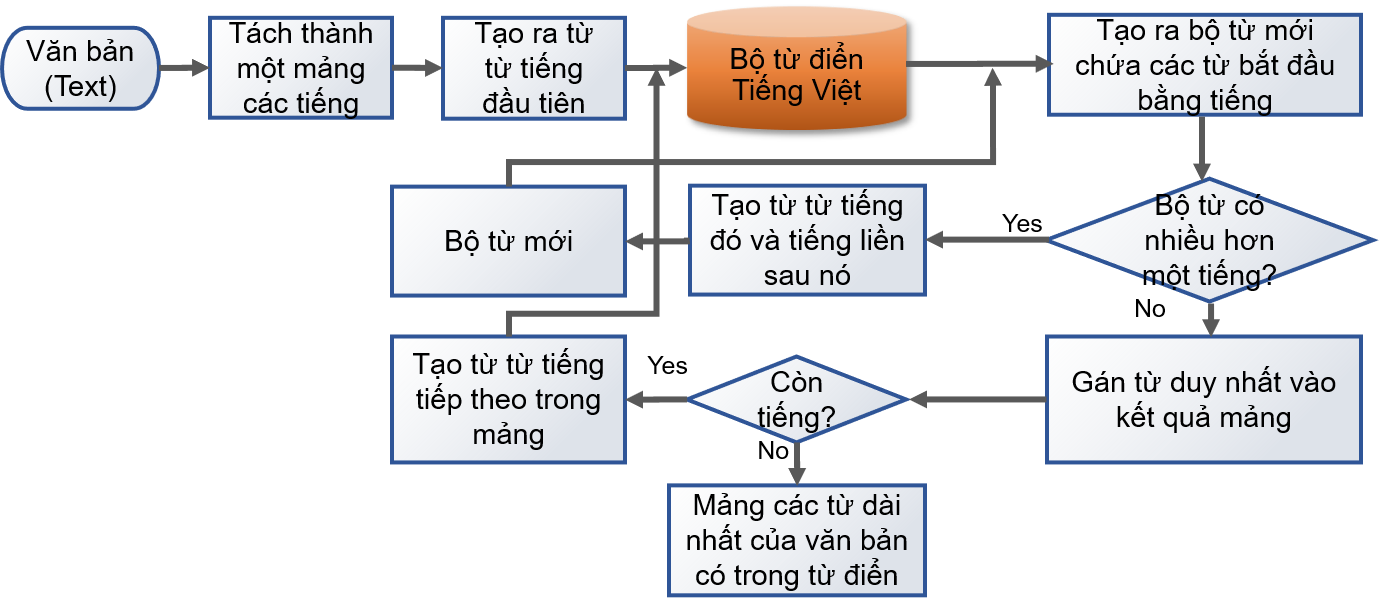
\includegraphics[width=10cm]{images/Diagram-longest-word.png}
    \caption{Tìm từ dài nhất}
    \label{fig:longest-word}
\end{figure}